\subsection{When does stochastic planning pay?}\label{sec:flex}\label{sec:sensitivity}

The modest VSS of the base case is a property of the cost structure, not of the method.
Same-day substitutes for scheduled capacity are only 60--80\% more expensive, and overtime can add 30\%.
We therefore vary the \emph{flexibility of recourse} on four regular days spread over the year:
\begin{itemize}
  \item the spot premium, from $1.4\times$ to $3.5\times$;
  \item the overtime cap, 30\% or 10\% of planned labour;
  \item the penalty for an unshipped unit, from \EUR{9} to \EUR{50}.
\end{itemize}
For each setting we compute the VSS and the reduction of the 95\% conditional value-at-risk (CVaR$_{95}$, the mean of the worst 5\% of days) on the true distribution.
In a second experiment (10 regular days) we repeat the forecast-based comparison of \cref{sec:value-forecast} under base and inflexible recourse.

\begin{table}[t]
\centering\small
\caption{Value of the stochastic solution as a function of recourse flexibility (means over four regular test days; SP and mean-value plans evaluated on 1000 true scenarios). $\Delta$CVaR$_{95}$: reduction of the expected cost of the worst 5\% of days achieved by the SP plan.}\label{tab:sensitivity}
\resizebox{\linewidth}{!}{\begin{tabular}{@{}rrrrrrrrrr@{}}\toprule
Spot & Overtime & Unmet & VSS & 95\% & VSS & Trucks & Crews & Unmet (\%) & $\Delta$CVaR$_{95}$ \\
premium & cap (\%) & penalty & \EUR{}/day & $\pm$ & \% & RP / EEV & RP / EEV & RP / EEV & \EUR{}/day \\ \midrule
1.4 & 10 & 15 & 4{,}382 & 199 & 0.17 & 553 / 576 & 284 / 286 & 0.09 / 0.09 & 19{,}216 \\
1.4 & 30 & 15 & 3{,}221 & 253 & 0.13 & 552 / 576 & 282 / 286 & 0.06 / 0.03 & -3{,}564 \\
1.8 & 10 & 15 & 3{,}654 & 203 & 0.15 & 569 / 578 & 284 / 286 & 0.14 / 0.12 & 19{,}666 \\
1.8 & 30 & 9 & 3{,}256 & 169 & 0.13 & 535 / 550 & 272 / 278 & 1.81 / 1.56 & 1{,}998 \\
1.8 & 30 & 15 & 2{,}552 & 164 & 0.10 & 572 / 578 & 282 / 286 & 0.10 / 0.05 & 1{,}835 \\
1.8 & 30 & 25 & 2{,}155 & 163 & 0.08 & 572 / 578 & 282 / 286 & 0.00 / 0.00 & 2{,}900 \\
1.8 & 30 & 50 & 2{,}183 & 209 & 0.08 & 571 / 578 & 282 / 286 & 0.00 / 0.00 & 5{,}257 \\
2.5 & 10 & 15 & 4{,}665 & 319 & 0.18 & 583 / 580 & 284 / 286 & 0.18 / 0.18 & 33{,}853 \\
2.5 & 30 & 15 & 3{,}435 & 161 & 0.14 & 582 / 580 & 282 / 286 & 0.15 / 0.10 & 10{,}690 \\
3.5 & 10 & 15 & 7{,}662 & 459 & 0.30 & 592 / 580 & 283 / 286 & 0.25 / 0.27 & 46{,}556 \\
3.5 & 30 & 15 & 5{,}688 & 262 & 0.23 & 592 / 580 & 282 / 286 & 0.20 / 0.19 & 25{,}113 \\
\bottomrule\end{tabular}
}
\end{table}

\begin{figure}[t]
  \centering
  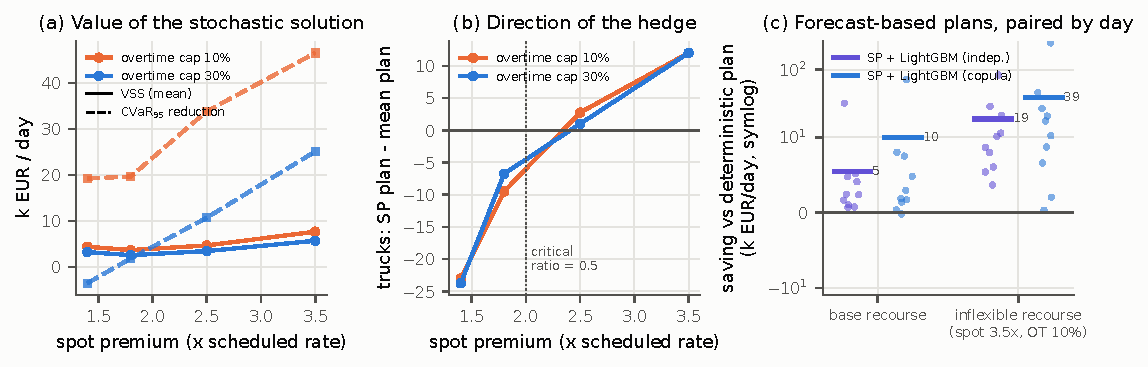
\includegraphics[width=\linewidth]{flex}
  \caption{(a) VSS (solid) and CVaR$_{95}$ reduction (dashed) against the spot premium, for two overtime caps. (b) Difference between the trucks planned by the SP and by the mean-value plan: the hedge changes sign where the newsvendor critical ratio crosses one half. (c) Daily saving of the forecast-based SP plans over the deterministic median plan, paired by day (bars: means).}
  \label{fig:flex}
\end{figure}

\Cref{tab:sensitivity,fig:flex} give a clear answer.
\begin{enumerate}
  \item \textbf{The value of stochastic planning grows with the cost of same-day flexibility.} The VSS triples, from \EUR{2.6}k to \EUR{7.7}k per day, between the base case and the inflexible case (spot $3.5\times$, overtime cap 10\%). The protection of the bad tail grows much faster: the SP plan lowers the CVaR$_{95}$ of the daily cost by \EUR{47}k per day in the inflexible case, against \EUR{2}k in the base case. When recourse is expensive, the stochastic plan is mainly an insurance against bad days.
  \item \textbf{The direction of the hedge follows newsvendor theory} (panel b). If $c$ is the per-unit price of scheduled capacity and $\gamma c$ that of its same-day substitute, under-provisioning costs $(\gamma-1)c$ per unit and over-provisioning $c$. The critical ratio $(\gamma-1)/\gamma$ is therefore below one half when $\gamma<2$. In that regime the SP buys \emph{fewer} trucks than the mean-value plan (up to 24 fewer at $\gamma=1.4$); above it, it buys \emph{more} (12 more at $\gamma=3.5$). A planner who always adds a safety margin is right only in the second regime.
  \item \textbf{Joint calibration pays when recourse is expensive} (panel c). With real LightGBM forecasts, the SP plans beat the deterministic median plan by \EUR{5}k (independent scenarios) and \EUR{10}k per day (copula) under base recourse. Under inflexible recourse they do so by \EUR{19}k and \EUR{39}k per day, on all 10 days. The copula's advantage over independent scenarios grows from \EUR{5}k to \EUR{20}k per day (better on 8 of 10 days). This resolves the null result of \cref{sec:value-forecast}. Dependence modelling matters exactly when the network cannot cheaply absorb a correlated, network-wide surprise.
  \item \textbf{The unshipped-unit penalty} has little effect on the VSS once it exceeds the cost of overtime plus spot (\EUR{15}--\EUR{50}). At \EUR{9} (\cref{sec:setting}) leaving 1.6--1.8\% of demand unshipped becomes the cheapest recourse, which we consider an unrealistic operating regime for a next-day network.
\end{enumerate}
